\documentclass[tikz, border=1cm]{standalone}

\begin{document}
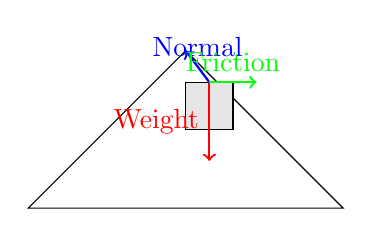
\begin{tikzpicture}

% Draw the inclined plane
\draw (-2,0) -- (2,0) -- (0,2) -- cycle;

% Draw the cube
\draw[fill=gray!20] (0,1) rectangle +(0.6,0.6);

% Force vectors
\draw[->,red,thick] (0.3,1.6) -- (0.3, 0.6) node[midway,left] {Weight}; % Weight
\draw[->,blue,thick] (0.3,1.6) -- (0,2) node[midway,above] {Normal}; % Normal force
\draw[->,green,thick] (0.3,1.6) -- (0.9,1.6) node[midway,above] {Friction}; % Frictional force

\end{tikzpicture}
\end{document}